\documentclass{article}

% Input packages & formatting
% Packages

% Math packages
\usepackage{amsmath} % Extended math functions
\usepackage{amssymb} % Extended math symbols (loads in amsfonts)
\usepackage{bm} % Bold math symbols
\usepackage{mathtools}

% Figure packages
\usepackage{caption} % Caption formatting for university standard
\usepackage{graphicx} % includegraphics command
\usepackage{subcaption} % Subfigures
\usepackage[section]{placeins} % Place floats in section
\usepackage{wrapfig}

% Table packages
\usepackage{booktabs} % Better tables
\usepackage{bigstrut} % Merged table cells
\usepackage{longtable} % Tables which overflow into next page
\usepackage{array}
\usepackage{colortbl} % Color table cells
\usepackage{makecell}
\usepackage{multirow}

% Fonts
\usepackage{lmodern} % Use latin modern rather than computer modern. Better for font encoding.
\usepackage[T1]{fontenc} % Allow text to be searchable in output

% Other packages
\usepackage{appendix} % Appendix environment
\usepackage{nextpage} % Cleartooddpage command
%\usepackage[square,comma,sort,numbers]{natbib} % Reference formatting
\usepackage{setspace} % Line spacing
\usepackage{listings} % Display code with syntax highlighting
\usepackage{upquote} % Vertical quotes in verbatim
\usepackage{xcolor} % Colors
\usepackage{titlesec} % Header spacing
\usepackage{xparse} % for tcolorbox
\usepackage[listings]{tcolorbox} % Colored boxes for highlighting syntax
\tcbuselibrary{breakable}
\tcbuselibrary{skins}
\usepackage{enumitem} % better enumerate/itemize options
\usepackage{fancyhdr}
\usepackage{multicol}
\usepackage{ifthen}
\usepackage{xstring}

% Table of contents
\usepackage{imakeidx} % Index page
\usepackage{tocloft} % Control of table of contents
\usepackage[nottoc]{tocbibind} % Adds bibliography, table of tables, table of figures, to table of contents
\usepackage[bookmarks,linktocpage,hidelinks]{hyperref} % Hyperlinks for sections, figures, etc.

% Formatting
% Page format
\setlength{\oddsidemargin}{0.00in}  % Left side margin for odd numbered pages
\setlength{\evensidemargin}{0.00in} % Right side margin for even numbered pages
\setlength{\topmargin}{0.00in}      % Top margin
\setlength{\headheight}{0.20in}     % Header height
\setlength{\headsep}{0.20in}        % Separation between header and main text
\setlength{\topskip}{0.00in}        % Top skip
\setlength{\textwidth}{6.50in}      % Width of the text
\setlength{\textheight}{8.50in}     % Height of the text
\setlength{\footskip}{0.50in}       % Foot skip
\setlength{\parindent}{0.00in}      % First line indentation
\setlength{\parskip}{6pt}        % Space between two paragraphs

% Captions (figures, tables, etc.)
\setlength{\floatsep}{\parskip}          % Space left between floats.
\setlength{\textfloatsep}{\floatsep}   % Space between last top float
% or first bottom float and the text
\setlength{\intextsep}{\floatsep}      % Space left on top and bottom
% of an in-text float
\setlength{\abovecaptionskip}{0.1in plus 0.25in}  % Space above caption
\setlength{\belowcaptionskip}{0.1in plus 0.25in}  % Space below caption
\setlength{\captionmargin}{0.50in}     % Left/Right margin for caption
\setlength{\abovedisplayskip}{0.00in plus 0.25in} % Space before Math stuff
\setlength{\belowdisplayskip}{0.00in plus 0.25in} % Space after Math stuff
\setlength{\arraycolsep}{0.10in}       % Gap between columns of an array
\setlength{\jot}{0.10in}                % Gap between multiline equations
\setlength{\itemsep}{0.10in}           % Space between successive items

% Counters (no section numbering)
\setcounter{tocdepth}{3}
\setcounter{secnumdepth}{0}

% Spacing
\setstretch{1.5}

\titlespacing*{\section}{0cm}{6pt}{6pt}[0cm]
\titlespacing*{\subsection}{0cm}{6pt}{6pt}[0cm]
\titlespacing*{\subsubsection}{0cm}{6pt}{6pt}[0cm]

\titleformat{\section}
{\sffamily\huge}{}{0pt}{\titlerule\vspace{-0.2cm}}
\titleformat{\subsection}
{\sffamily\itshape\Large}{}{0pt}{}

% Macro for syntax
\newtcolorbox{syntax}{
    size=small,
    sharp corners,
    colframe=black,
    colback=yellow,
    fontupper=\bfseries\ttfamily
}

% Macro for argument table
\newenvironment{args}{
    \begin{tabular}{>{\bfseries\ttfamily}p{0.25\linewidth} p{0.69\linewidth}}
    }{
    \end{tabular}\par
    \vspace{0.5\baselineskip}
}

% Note: Requires packages "listing", "xcolor", and "textcomp"
\lstdefinelanguage{verbatim}{
    basicstyle=\ttfamily\small,
    xleftmargin=9pt,
    xrightmargin=9pt,
    columns=fullflexible,
    keepspaces=true,
    breaklines=true
}

% Example code
\AtBeginDocument{
\newtcolorbox[blend into=listings]{example}[2][]{
    colback=blue!3!white,
    colframe=black,
    colbacktitle=blue!15!white,
    coltitle=black,
    sharp corners,
    enhanced,
    breakable,
    size=small,
    before upper={
        \setstretch{1.0}\lstset{language=verbatim}\vspace{3pt}\textsf{\textit{Code:}}
    },
    subtitle style={
        colback=blue!20!white,
        fonttitle=\sffamily
    },
    before lower={
        \setstretch{1.0}\lstset{language=verbatim}\vspace{3pt}\textsf{\textit{Output:}}
    },
    fonttitle=\sffamily,
    title={#2},
    #1
}
}

% Links to sub and subsub commands - optional boolean argument, default true. if false, only displays subcmd.

% Commands (and command ensembles)
\newcommand{\command}[1]{\protect\hypertarget{#1}{#1}\index{#1}}
\newcommand{\subcommand}[2]{\protect\hypertarget{#1 #2}{#1 #2}\index{#1!#2}}
\newcommand{\cmdlink}[1]{\protect\hyperlink{#1}{\textit{#1}}}
\newcommand{\subcmdlink}[3][1]{\protect\hyperlink{#2 #3}{\ifnum#1=1\relax\textit{#2 #3}\else\textit{#3}\fi}}

% Methods (first arg is class)
\newcommand{\method}[2]{\protect\hypertarget{$#1Obj #2}{\$#1Obj #2}\index{#1 methods!#2}}
\newcommand{\methodlink}[3][1]{\protect\hyperlink{$#2Obj #3}{\ifnum#1=1\relax\textit{\$#2Obj #3}\else\textit{#3}\fi}}

% Macros for figure/table names
\newcommand{\fig}{\figurename\ }
\newcommand{\figs}{\figurename s }
\newcommand{\tbl}{\tablename\ }
\newcommand{\tbls}{\tablename s }
\newcommand{\eq}{Eq. }
\newcommand{\eqs}{Eqs. }
\renewcommand{\lstlistingname}{Example}% Listing -> Example
\renewcommand{\lstlistlistingname}{List of \lstlistingname s}% List of Listings -> List of Examples
\newcommand{\ex}{Example }
\newcommand{\exs}{Examples }
\newcommand{\var}[1]{\texttt{\textbf{\$#1}}}

% Header/footer
\renewcommand{\headrulewidth}{0pt}

% Changes to hyperlinks (URLs)
\renewcommand\UrlFont{\color{blue}\rmfamily}

% New column type 
% https://tex.stackexchange.com/questions/75717/how-can-i-mix-itemize-and-tabular-environments
\newcolumntype{L}{>{\labelitemi~~}l<{}}
\newcommand{\version}{1.0.1}

\renewcommand{\cleartooddpage}[1][]{\ignorespaces} % single side
\newcommand{\caret}{$^\wedge$}

% Other macros
\renewcommand{\^}[1]{\textsuperscript{#1}}
\renewcommand{\_}[1]{\textsubscript{#1}}

\title{\Huge Flytrap: Tcl Debugging Tools\\\small Version \version}
\author{Alex Baker\\\small\url{https://github.com/ambaker1/flytrap}}
\date{\small\today}
\begin{document}
\maketitle
\begin{abstract}
\begin{center}
Say goodbye to debugging with countless \textit{puts} statements, and say hello to ``flytrap''!
\end{center}
\end{abstract}
\clearpage
\section{Pausing a Script} 
The \cmdlink{pause} command pauses a Tcl script, prints the file and line number, and enters command-line mode, allowing the user to query variables and insert code into an analysis. 
If the command entered while paused returns an error, the error message will be displayed and the script will remain paused. 
If the command entered is ``return'', the pause will be exited and the corresponding result and options will be passed to the caller. 
For example, a loop can be broken by entering \textit{return -code break} in pause mode. 
Pressing enter with no commands will simply continue the script.
\begin{syntax}
\command{pause} <\$frameOffset>
\end{syntax}
\begin{args}
\$frameOffset & Frame offset for calling pause in another level (e.g. uplevel) Default 0. 
\end{args}
\begin{example}{Pausing an analysis}
\begin{lstlisting}
pause
\end{lstlisting}
\tcblower
\begin{lstlisting}
PAUSED...
(line 407 file "C:/User/Documents/MyFile.tcl")
> 
\end{lstlisting}
\end{example}
Note: If in interactive mode, there may not be a file to pause in. 
In this case, it will list the procedure or script where the pause occurred.
\clearpage
\section{Advanced Tcl Debugger}
The \cmdlink{flytrap} command parses a Tcl script, and prints out the evaluation steps and results if an error is reached.
Additionally, if an error is reached, the script will pause at the line where the error occurred, allowing for interactive introspection of the problem, at the depth specified.
\begin{syntax}
\command{flytrap} <-depth \$maxDepth> <-verbose \$verboseFlag> (-file \$filename | <-body> \$body) 
\end{syntax}
\begin{args}
\$maxDepth & Optional recursive depth to step into procedures (default 0). \\
\$verboseFlag & Optional flag to always print out all steps and results (default 0). \\
\$filename & File path of Tcl script to debug. Mutually exclusive with -body. \\
\$body & Tcl script to debug. Mutually exclusive with -file.
\end{args}

\begin{example}{Verbose evaluation of a procedure}
\begin{lstlisting}
proc add {a b} {
    return [expr {$a + $b}]
}
set a 5
set b 7
flytrap -depth 1 -verbose true -body {
    add [expr {$a*2}] $b
}
\end{lstlisting}
\tcblower
\begin{lstlisting}
> expr {$a*2}
10
> add 10 7
  > expr {$a + $b}
  17
  > return 17
  17
17
\end{lstlisting}
\end{example}
\clearpage
\section{Printing Variables to Screen} 
The \cmdlink{printVars} command is a short-hand function for printing the name and values of Tcl variables, in the same style as the Tcl \textit{parray} command.
\begin{syntax}
\command{printVars} \$name1 \$name2 …
\end{syntax}
\begin{args}
\$name1 \$name2 … & Name(s) of variables to print
\end{args}

\begin{example}{Printing variables to screen}
\begin{lstlisting}
set a 5
set b 7
set c(1) 5
set c(2) 6
printVars a b c
\end{lstlisting}
\tcblower
\begin{lstlisting}
a = 5
b = 7
c(1) = 5
c(2) = 6
\end{lstlisting}
\end{example}
\clearpage
\section{Variable Viewer Widget Class}
The class \cmdlink{varViewer} is a TclOO class that creates widget objects that display the values of variables. 
It can be used to monitor variable values in a widget. 
\begin{syntax}
\command{varViewer} new \$varList <\$title> \\
varViewer create \$name \$varList <\$title> 
\end{syntax}
\begin{args}
\$name & Object name. \\
\$varList & List of variables to view. \\
\$title & Optional title. Default ``Workspace''.
\end{args}
\begin{example}{Monitoring variable values}
\begin{lstlisting}
set i 0
varViewer new i {counter}
for {set i 0} {$i < 1000} {incr i} {
    update
}
\end{lstlisting}
\end{example}

The command \cmdlink{viewVars} opens up a \cmdlink{varViewer} widget displaying the values of all the variables in the current scope, and then pauses the script using the \cmdlink{pause} command, such that continuing destroys the widget. 
\begin{syntax}
\command{viewVars} 
\end{syntax}
\begin{example}{Workspace viewer}
\begin{lstlisting}
set a 5
set b 7
array set c {1 5 2 6}
viewVars
\end{lstlisting}
\tcblower

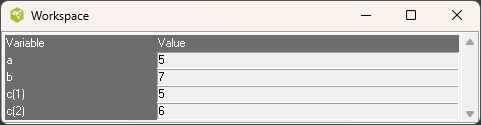
\includegraphics[width = 4in]{figures/workspace.png}
\end{example}
\end{document}
